% !TeX spellcheck = en_GB

% ------------------------------- %
%% Random Forest Classifier %%
% ------------------------------- %

\begin{frame}{Random Forest for Classification}

{\footnotesize Package \texttt{\{randomForest\}}\vspace{-1ex}
\begin{itemize}\setlength{\itemsep}{-0.5ex}
	\item \texttt{randomForest(formula, data={\color{blue}NULL}, ntree={\color{red}500}, mtry={\color{blue}sqrt}(p), importance={\color{red}TRUE}, \dots)}
	\item \texttt{importance(x, type={\color{blue}NULL}, class={\color{blue}NULL}, \dots)}
    \item \texttt{varImpPlot(x, sort={\color{red}TRUE}, \dots)}
    \item \texttt{x\$confusion}
    \item \texttt{x\$err.rate}
\end{itemize}}

{\texttt{x}} is a {\texttt{randomForest}} object;

{\texttt{ntree}} = number of trees grown;

{\texttt{p}} = number of predictors;

{\texttt{mtry}} = number of predictors sampled for splitting at each node.

\end{frame}

% ------------------------------- %

\begin{frame}{OOB Error}
\begin{columns}
\begin{column}{0.35\textwidth}

{\footnotesize \begin{itemize}
    \item p = 8
    \item mtry = $\sqrt{p} \simeq 2.83$ 
    \item OOB estimate error rate: $24.41\%$
\end{itemize}}

\end{column}
\begin{column}{0.75\textwidth}
\begin{figure}
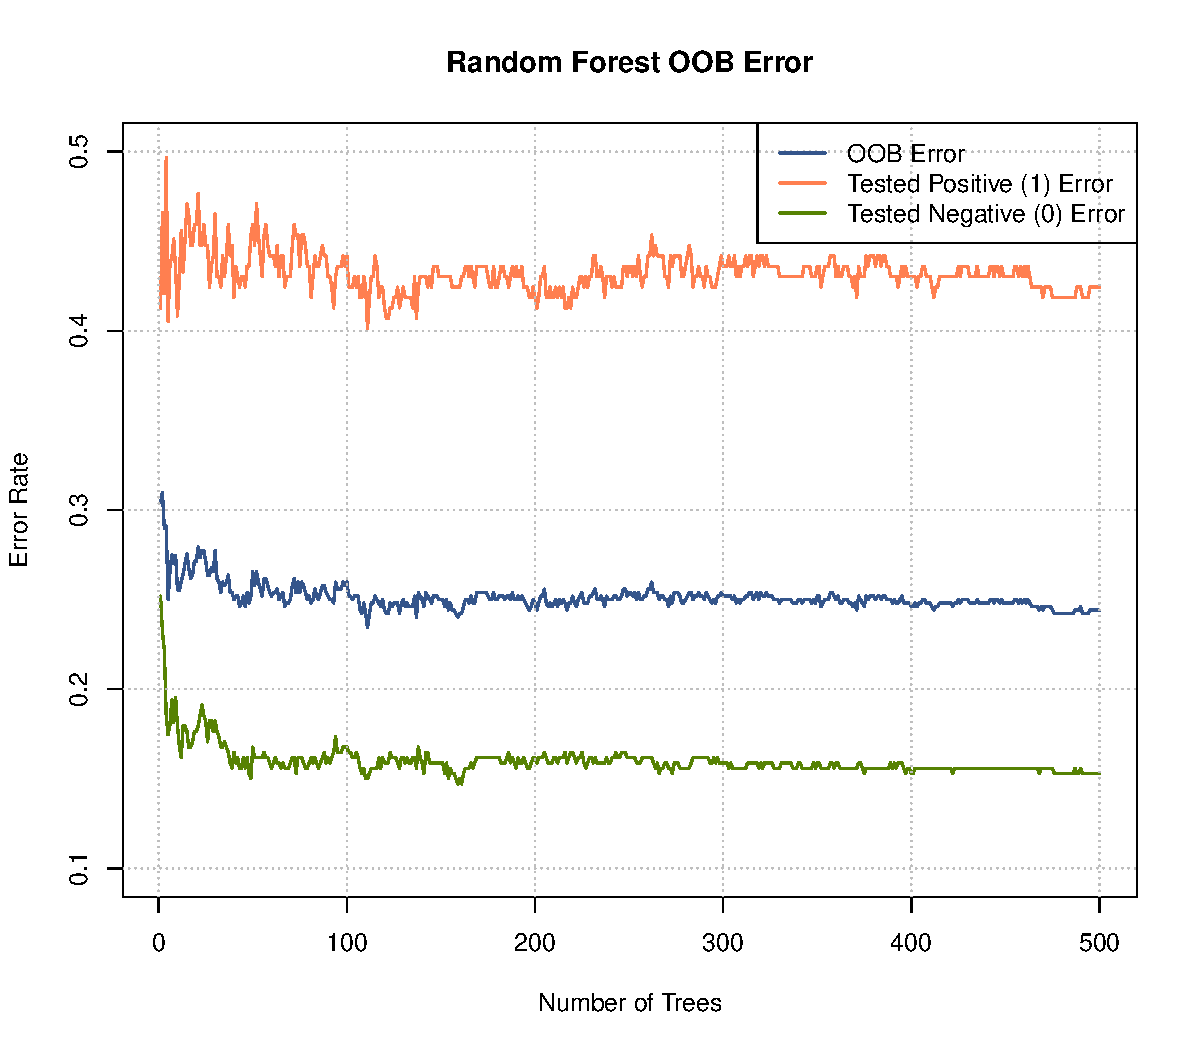
\includegraphics[width=1.05\columnwidth]{diabete_forest_error.pdf}
\end{figure}
\end{column}
\end{columns}
\end{frame}

% ------------------------------- %

\begin{frame}{Optimal OOB Error}

\begin{columns}
\begin{column}{0.35\textwidth}
{\footnotesize \begin{itemize}
    \item p = 8
    \item mtry = 4 
    \item min OOB estimate error rate: $22.85\%$
\end{itemize}}

\end{column}
\begin{column}{0.75\textwidth}
\begin{figure}
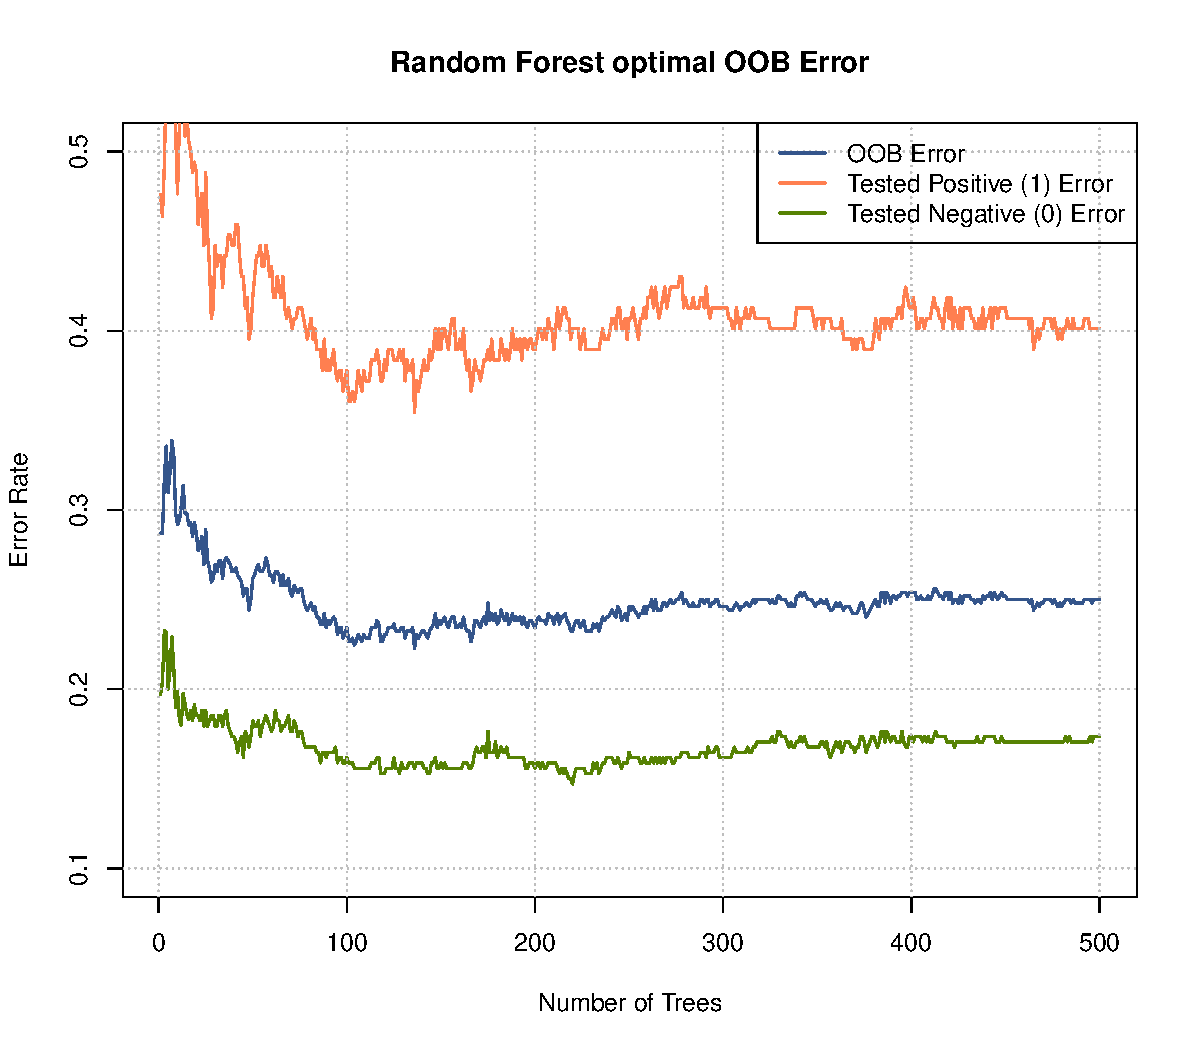
\includegraphics[width=1.05\columnwidth]{diabete_forest_error_opt.pdf}
\end{figure}
\end{column}
\end{columns}

\end{frame}

% ------------------------------- %

\begin{frame}{Variable importance}

\begin{figure}
	\hspace*{-2.5em}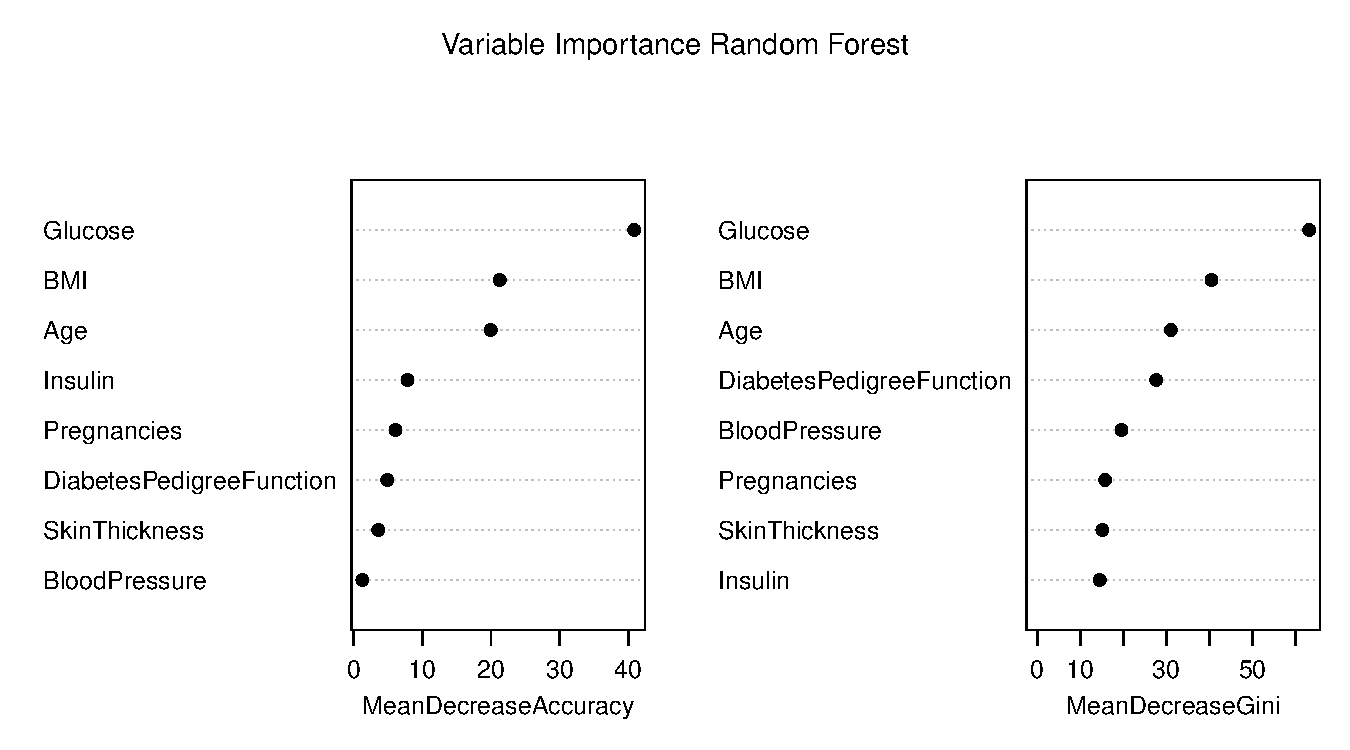
\includegraphics[width=1.15\textwidth,trim=0 0 0 1.5cm,clip]{./Figures/diabete_var_imp.pdf}
\end{figure}

\end{frame}
